\subsubsubsubsection{Parser}
\begin{figure}[h]
\centering
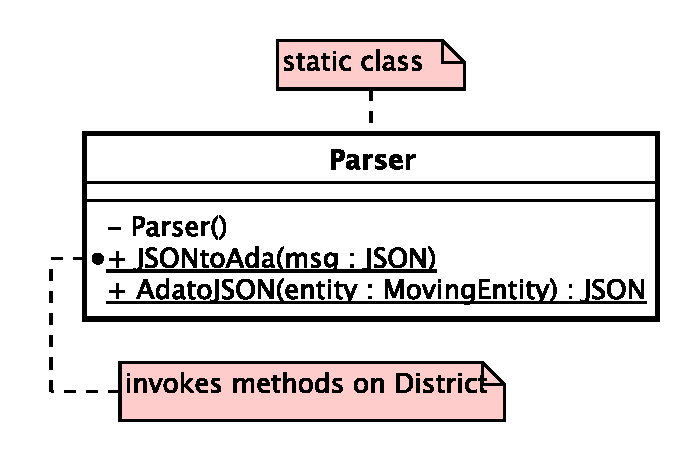
\includegraphics[scale=0.6,keepaspectratio]{images/solution/parser.eps}
\caption{App::Interface::Parser}
\label{fig:sd-app-parser}
\end{figure}
\FloatBarrier
\begin{itemize}
  \item \textbf{Description} \\
    It represents a parser which converts JSON messages to Ada statements and vice versa.
  \item \textbf{Attribute}
  \begin{itemize}
    \item \texttt{- district: District} \\
The district object used as facade for the application layer.
  \end{itemize}
  \item \textbf{Operation}
  \begin{itemize} 
    \item \texttt{+ JSONtoAda(msg: JSON)} \\
Converts the JSON message to Ada statements invoking district.
    \item \texttt{+ AdatoJSON(entity: MovingEntity) : JSON} \\
Converts a moving entity into a JSON message returning the message as result.
  \end{itemize}
\end{itemize}
